\section{Programming part}
\subsection{Question 1}
Yes, there will be no problem in making a peer-to-peer connection between
peer $A$ and peer $B$.

\begin{lstlisting}
peer A (alice) <--> ns: HELLO alice alice_port
ns  <--> peer A (alice): 100 CONNECTED

peer A (alice) <--> ns: LOOKUP bob
ns  <--> peer A (alice): 200 INFO bob_ip bob_port

peer A (alice) <--> peer B (bob): HELLO alice
peer B (bob) <--> peer A (alice): 100 CONNECTED

peer A (alice) <--> peer B (bob): MSG Are you single
\end{lstlisting}

\subsection{Question 2}
It is not prudent to keep unused connections open, it just take up system
resources. On the other hand connections should be keep open to connections
that are used often, besacuse the the whole connection and disconnection
process add a certen overhead to a continuous transmission.

We would suggest implementing a timeout, such that connections are idle only
for a certen amount of time before they are automaticly closed. This way only
active connections take up resources in the long run.


\subsection{Question 3}
We suggest a design where a peer is working as group accountend, and the name
server only knows which peer is authorized to act as group master.

Peers would be able to lookup and list the groups on the name server and
thereafter connect to the peer hosting the list of group members.

The peer working as group master, would then send updates regarding members to
all of its group members(peers joining and leaving the group).

All peers - which are members of the group - will then have an updated list of
group members and could use use a group-broadcast method to send messages to
other group memebers.

On the name server we would need
\begin{lstlisting}
ADDGROUP <groupname>
DELGROUP <groupname>
LISTGROUPS <groupname>
LOOKUPGROUP <groupname>
\end{lstlisting}

On the peer side we would need
\begin{lstlisting}
ADD_ME_TO_GROUP <nick> <port>
DEL_ME_FROM_GROUP

ADD_GROUP_MEMBER <nick> <port>
DEL_GROUP_MEMBER <nick>

MSG_GROUP <group> <msg>
\end{lstlisting}

\subsection{Question 4}
We can achieve this with flooding. Figure 2, shows how $u0$ is broadcasting to the rest of the network
consistng of $u1,u2,u3,u4,u5,u6$.

$u0$ takes the broadcast-list and splits it in half, then $u0$ sends the message
and the remaining of the two new half broadcasting lists (the reciever is subtracted) to first
member of the lists.

This implies that $u1$ will get the message and the broadcast list $u2, u3$ and $u4$ will get the message and the list $u5,u6$.

$u1$ splits the remaning list in two and because each list now only contains
one peer, only the message is send to $u2$ and $u3$. The exact same procedure
is followed by $u4$. As mentioned above a graphical illustration is shown in Figure 2.

\begin{figure}[!h]
    \centering
    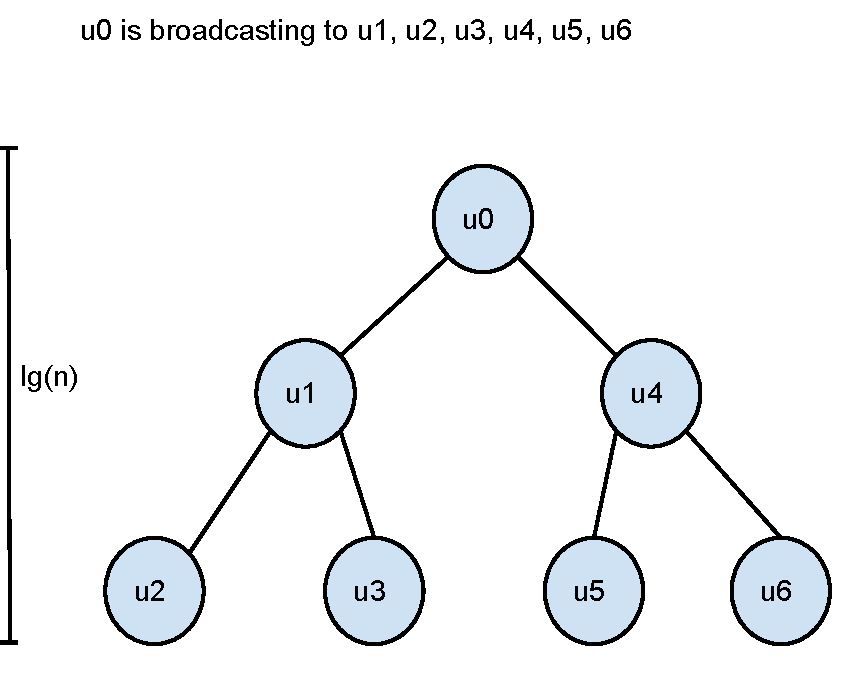
\includegraphics[width=10cm]{graphics/flooding}
    \caption{Flooding messages}
\end{figure}



\subsection{Name Server Extentions}
